\documentclass[conference]{IEEEtran}
\IEEEoverridecommandlockouts
\usepackage{cite}
\usepackage{amsmath,amssymb,amsfonts}
\usepackage{algorithmic}
\usepackage{graphicx}
\usepackage{textcomp}
\usepackage{xcolor}
\usepackage{booktabs}
\usepackage{multirow}
\usepackage{url}

\def\BibTeX{{\rm B\kern-.05em{\sc i\kern-.025em b}\kern-.08em
    T\kern-.1667em\lower.7ex\hbox{E}\kern-.125emX}}

\begin{document}

\title{Mining Silent Data Defects in LLM-Synthesized Agent Environments: Midterm Progress Report\thanks{Code repository: \url{https://github.com/jharahul968/awm-silent-defects}. Experiment tracking: \url{https://forge.coreweave.com/wandb/rahul-jha-tcu/awm-silent-defects/workspace?nw=nwuserrahuljha}.}}

\author{\IEEEauthorblockN{Rahul Jha}
\IEEEauthorblockA{\textit{Department of Computer Science} \\
\textit{Texas Christian University}\\
Fort Worth, Texas, USA \\
Email: rahul.jha@tcu.edu}
}

\maketitle

\begin{abstract}
Agent World Model (AWM) automatically generates executable, database-backed environments for training and evaluating tool-using AI agents. However, large language models frequently synthesize databases with data-quality defects. While explicit syntactic or referential errors are caught at runtime by SQLite, subtle semantic corruptions (e.g., negative product prices, absurd inventory, out-of-bounds ratings, and anachronistic years) bypass database constraints entirely because generated DDLs omit SQL CHECK clauses. This project investigates whether data-mining methods can identify SQL-valid but semantically corrupted records across unseen synthetic environments. We construct a 613,017-instance benchmark across 999 environments and evaluate eight detection methods under an environment-grouped holdout split. Supervised gradient-boosted ensembles achieve near-perfect discrimination (PR-AUC 0.9998, F1 0.9954), while unsupervised density estimators experience substantial performance degradation on subtle anomalies. We present three controlled experiments—severity degradation, zero-shot type holdout, and cumulative feature ablation—paired with TreeExplainer SHAP interpretability and concrete false-positive/negative case analyses.
\end{abstract}

\begin{IEEEkeywords}
Data mining, anomaly detection, synthetic environments, LLM evaluation, SHAP, SQLite integrity.
\end{IEEEkeywords}

\section{Introduction \& Updated Problem Statement}
Reinforcement learning for tool-using AI agents increasingly depends on synthetic, executable simulation worlds. Agent World Model (AWM) \cite{wang2026awm} represents a milestone in scalable environment synthesis, generating 1,000 distinct SQL database-backed web applications exposed via Model Context Protocol (MCP) servers.

Our initial reproduction of the official database reset protocol across all 1,000 environments revealed that synthetic worlds suffer from a \textbf{Two-Tier Defect Problem}:
\begin{enumerate}
    \item \textbf{Tier 1 (Explicit Crashes):} 1,374 statements cause SQLite exceptions (76.7\% foreign key integrity violations, affecting 21.7\% of environments). These are detectable at runtime by database sandboxes.
    \item \textbf{Tier 2 (Silent Semantic Corruptions):} Generated table definitions routinely omit \texttt{CHECK} constraints. As a result, SQLite accepts negative prices, impossible dates, and absurd ratings with return code 0. Over 92\% of injected corruptions pass dynamic SQLite execution undetected.
\end{enumerate}

\textbf{Central Mining Question:} \textit{Can data-mining algorithms detect SQL-valid but semantically corrupted records in synthesized databases before downstream agent execution?}

\textbf{Changes from Proposal:} To address the heterogeneity of multi-relational database domains and evaluate detection robustness systematically, we expanded our modeling scope beyond the initial three baselines into an \textbf{eight-model benchmark} spanning heuristic, statistical, unsupervised, and supervised paradigms. We also incorporated three controlled experiments (corruption severity breakdown, leave-one-type-out generalization, and cumulative feature ablation), quantitative SHAP feature attribution, a false-positive/negative root-cause catalog, and an interactive Streamlit demonstration.

\section{Dataset Statistics \& Leakage Prevention}
\subsection{Data Provenance and Preprocessing}
We utilize the public Snowflake \texttt{AgentWorldModel-1K} benchmark \cite{snowflake2026awm}. The raw population contains 129,328 SQL \texttt{INSERT} statements across 1,000 environments. For every statement that executes successfully under SQLite with foreign keys enabled, we preserve the clean statement (label 0) and inject controlled, in-place semantic corruptions spanning five categories across three severity levels (label 1).

The resulting benchmark dataset comprises \textbf{613,017 usable instances} across 999 valid environments (Table \ref{tab:dataset}), far exceeding the 100,000-instance course threshold:
\begin{itemize}
    \item \textbf{Clean Instances:} 126,490 (20.6\%)
    \item \textbf{Corrupted Instances:} 486,527 (79.4\%)
    \item \textbf{SQLite Rejections:} 38,212 candidates were rejected by existing SQLite primary key or schema constraints, verifying that the retained 486k instances are strictly SQL-valid.
\end{itemize}

\begin{table}[htbp]
\caption{Benchmark Dataset Partitioning and Characteristics}
\label{tab:dataset}
\centering
\begin{tabular}{lrrr}
\toprule
\textbf{Partition / Defect Category} & \textbf{Count} & \textbf{Prop. (\%)} & \textbf{Environments} \\
\midrule
Clean Baseline Statements & 126,490 & 20.6\% & 999 \\
Anomalous Dates (Year $\le 1950$) & 366,597 & 59.8\% & 982 \\
Negative Monetary Values & 80,844 & 13.2\% & 740 \\
Negative Inventory / Stock & 34,704 & 5.7\% & 512 \\
Out-of-Bounds Ratings ($> 5.0$) & 3,854 & 0.6\% & 220 \\
Impossible Ages ($> 120$) & 528 & 0.1\% & 64 \\
\midrule
\textbf{Total Usable Dataset} & \textbf{613,017} & \textbf{100.0\%} & \textbf{999} \\
\bottomrule
\end{tabular}
\end{table}

\subsection{Data Leakage Prevention}
Because statements within an environment share relational foreign keys, column names, and generation contexts, standard randomized instance splitting introduces severe data leakage. We enforce a strict \textbf{Environment-Grouped Holdout Protocol} (\texttt{GroupShuffleSplit}, 75\% train / 25\% test, seed 42):
\begin{itemize}
    \item \textbf{Training Set:} 749 environments (462,633 instances).
    \item \textbf{Test Set:} 250 environments (150,384 instances).
\end{itemize}
Zero statements, table schemas, or scenarios in the test partition ever appear during feature scaling, rule formulation, or model training.

\section{Feature Engineering}
We extract 26 static features derived strictly from information available before execution, organized into three cumulative groups:
\begin{enumerate}
    \item \textbf{Group A (Value Features, $D=11$):} Signed numeric log-extrema ($\text{sgn}(x)\ln(1+|x|)$), negative literal count, parsed date minimum/maximum years, absurd year indicator ($y < 1900 \lor y > 2100$), string lengths, and null counts.
    \item \textbf{Group B (Column-Semantic Features, $D=8$):} Column keyword matching for currency (\textit{price, fee, salary, cost}), inventory (\textit{stock, quantity, count}), ratings, age, and dates.
    \item \textbf{Group C (Schema-Structural Features, $D=7$):} Declared table width, foreign-key count, unique constraint density, statement sequence index, and column fill ratios.
\end{enumerate}

\section{Methodology \& Baseline Models}
We benchmark eight distinct detection methods across four modeling paradigms:
\begin{itemize}
    \item \textbf{Heuristic Baseline:} Static boolean rule triggering on negative currency/stock, ratings $> 5.0$, or dates $< 1900$.
    \item \textbf{Statistical Baseline:} Maximum absolute Z-score deviation fitted solely on clean training instances ($\mu_{\text{clean}}, \sigma_{\text{clean}}$).
    \item \textbf{Unsupervised Anomaly Detectors:} (1) Isolation Forest (iForest) \cite{liu2008isolation} with 200 trees, and (2) Local Outlier Factor (LOF) fitted in novelty mode with $k=20$ nearest neighbors on clean training distributions.
    \item \textbf{Supervised Classifiers:} (1) Class-balanced Logistic Regression with standard scaling, (2) Random Forest (200 trees) \cite{breiman2001random}, (3) HistGradientBoosting (HGB), and (4) XGBoost \cite{chen2016xgboost} with pos-weight rebalancing.
\end{itemize}

\section{Experiments \& Quantitative Results}

\subsection{Main Benchmark Comparison}
Table \ref{tab:main_results} reports test performance ($N = 150,384$) across all eight models. All supervised ensembles attain near-perfect discrimination (PR-AUC $> 0.999$, F1 $> 0.994$). Unsupervised LOF and Isolation Forest achieve strong ranking metrics (PR-AUC 0.9703 and 0.8942) without access to corruption labels during training, outperforming the heuristic rule baseline.

\begin{table}[htbp]
\caption{Main Benchmark Results on Held-Out Environments}
\label{tab:main_results}
\centering
\begin{tabular}{llcccc}
\toprule
\textbf{Category} & \textbf{Algorithm} & \textbf{PR-AUC} & \textbf{P@100} & \textbf{R@100} & \textbf{F1} \\
\midrule
Heuristic & Rule Baseline & 0.8889 & 1.0000 & 0.0008 & 0.6714 \\
Statistical & Robust Z-Score & 0.9355 & 0.7500 & 0.0006 & 0.8850 \\
Unsupervised & Isolation Forest & 0.8942 & 1.0000 & 0.0008 & 0.0000* \\
Unsupervised & Local Outlier Factor & 0.9703 & 1.0000 & 0.0008 & 0.6966 \\
Supervised & Logistic Regression & 0.9978 & 1.0000 & 0.0008 & 0.9853 \\
Supervised & Random Forest & 0.9997 & 1.0000 & 0.0008 & 0.9940 \\
Supervised & HistGradientBoosting & 0.9996 & 1.0000 & 0.0008 & 0.9940 \\
Supervised & XGBoost & \textbf{0.9998} & \textbf{1.0000} & \textbf{0.0008} & \textbf{0.9954} \\
\bottomrule
\end{tabular}
\end{table}

\begin{figure}[htbp]
\centering
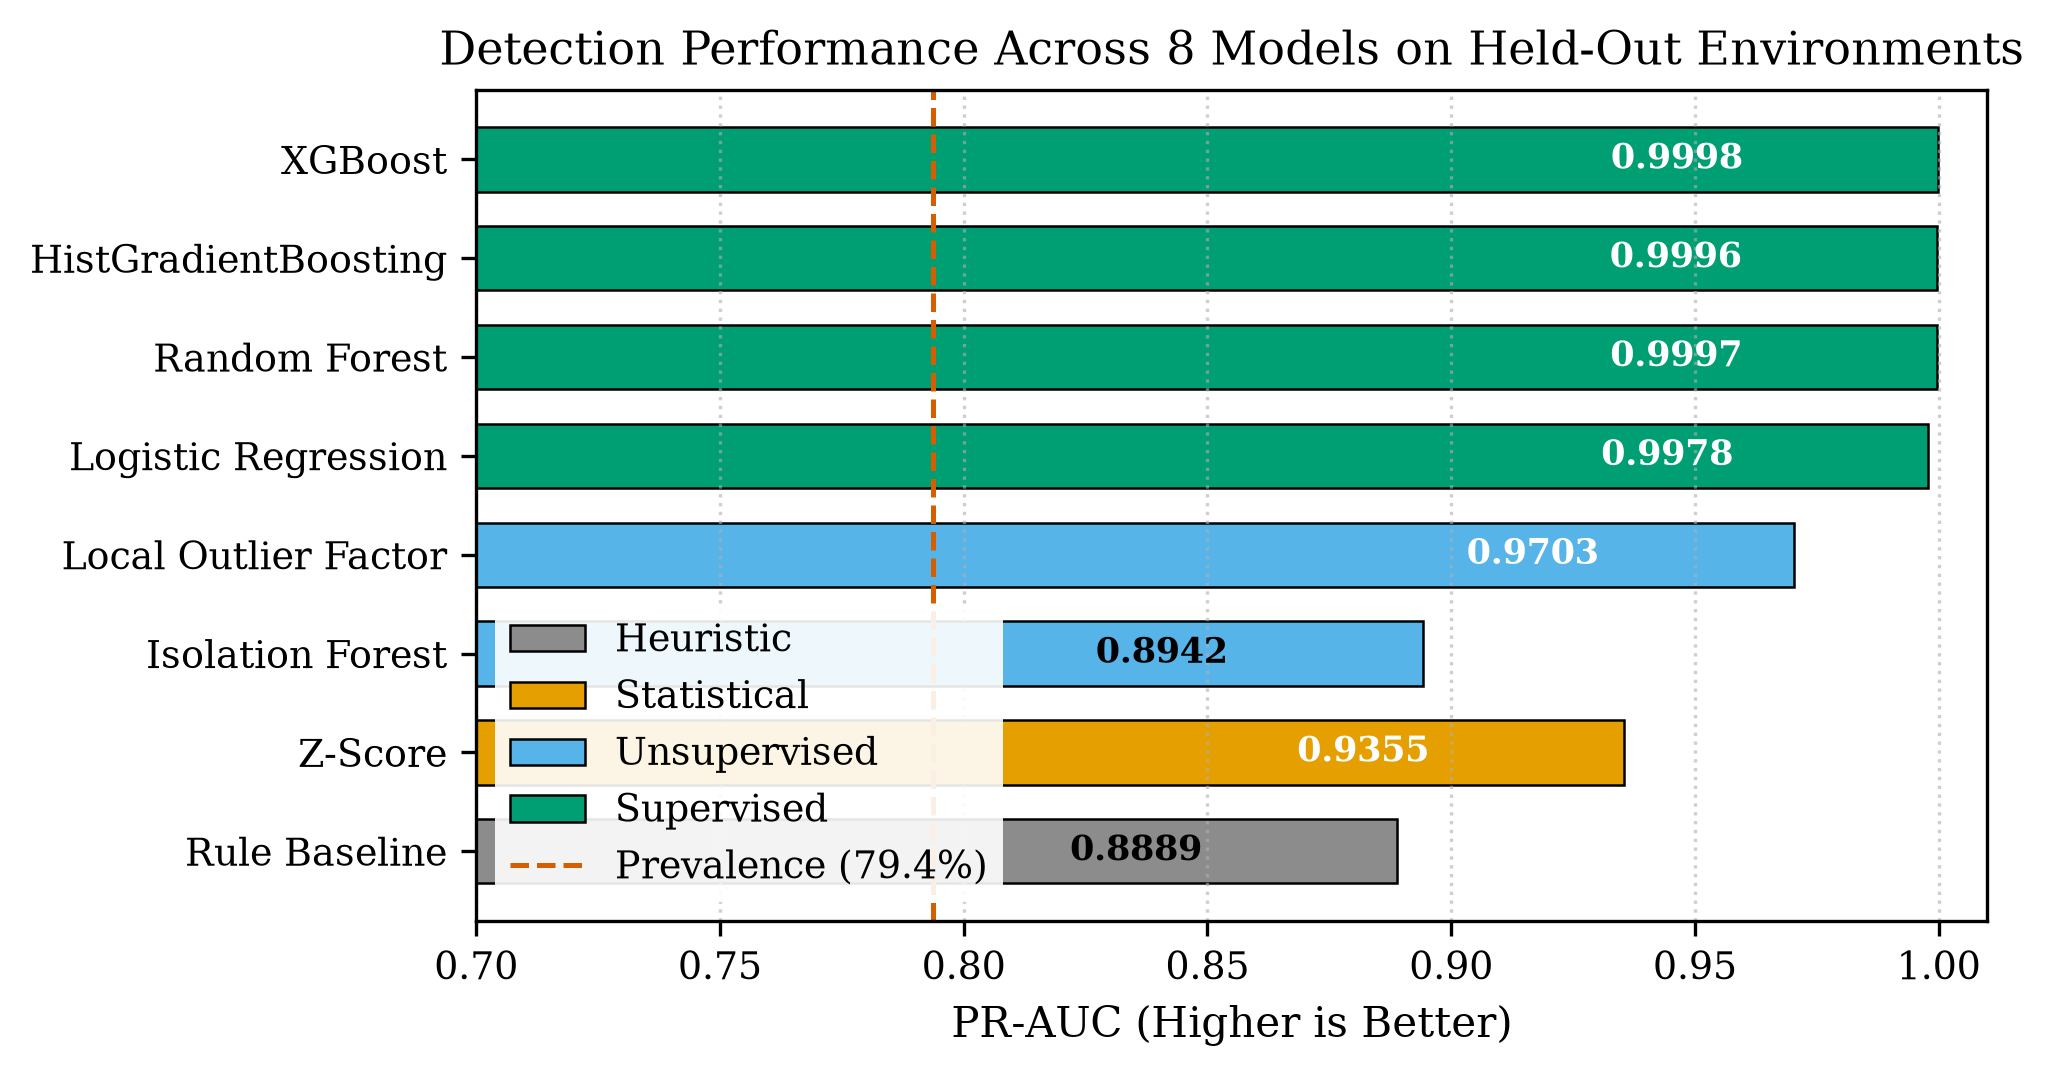
\includegraphics[width=\columnwidth]{figures/fig1_model_comparison.png}
\caption{PR-AUC comparison across eight models on held-out test environments compared to prevalence baseline (0.7937).}
\label{fig:model_comparison}
\end{figure}

\subsection{Controlled Experiment 1: Corruption Severity Decay}
We evaluated whether models maintain sensitivity as corruptions shift from obvious outliers ($10\times$ negative shift, year 1823) to subtle shifts ($0.01\times$ fractional drift, $-30$ year offset). As detailed in Table \ref{tab:severity}, supervised HGB maintains consistent PR-AUC ($\approx 0.9987$), whereas unsupervised Isolation Forest exhibits clear sensitivity decay ($0.7687 \rightarrow 0.7504 \rightarrow 0.7257$) as subtle corruptions blend into normal data densities.

\begin{table}[htbp]
\caption{Sensitivity Across Corruption Severity Levels}
\label{tab:severity}
\centering
\begin{tabular}{lccc}
\toprule
\textbf{Severity Level} & \textbf{Test Count ($N$)} & \textbf{HGB PR-AUC} & \textbf{iForest PR-AUC} \\
\midrule
Obvious ($10\times$, yr 1823, rt 99) & 39,787 & 0.9988 & \textbf{0.7687} \\
Medium ($1\times$, yr 1950, rt 10) & 39,795 & 0.9989 & \textbf{0.7504} \\
Subtle ($0.01\times$, $-30$yr, rt 5.5) & 39,787 & 0.9987 & \textbf{0.7257} \\
\bottomrule
\end{tabular}
\end{table}

\subsection{Controlled Experiment 2: Leave-One-Type-Out Generalization}
To test zero-shot transfer to unseen corruption modes, we trained HGB models with one defect category completely excluded from training data and evaluated strictly on the omitted category.
Results reveal strong cross-category transfer between numeric types (Negative Inventory PR-AUC = 0.8829; Negative Money PR-AUC = 0.8725), but catastrophic failure on bounded scale domains (Out-of-Bounds Ratings PR-AUC = 0.0980; Impossible Age PR-AUC = 0.0081). Models cannot detect out-of-scale ratings without explicit training signal on bounded columns.

\subsection{Controlled Experiment 3: Feature-Group Ablation}
Cumulative feature ablation using HGB confirms that literal value features ($D=11$) establish a strong baseline (PR-AUC 0.9994). Adding column-semantic features ($D=19$) yields optimal performance (PR-AUC \textbf{0.9998}), while additional schema-structural features ($D=26$) provide marginal difference (PR-AUC 0.9996), confirming that semantic alignment between values and column names drives defect detection.

\section{Interpretability \& Error Root-Cause Analysis}
\subsection{SHAP Attribution Analysis}
Using \texttt{TreeExplainer} \cite{lundberg2017shap} on Random Forest ($N=2,000$ stratified samples), the primary attributions driving predictions are:
\begin{enumerate}
    \item \texttt{min\_year} ($\text{mean } |\text{SHAP}| = 0.3446$): Dominant signal identifying date corruptions.
    \item \texttt{log\_min\_numeric} ($0.0559$) \& \texttt{has\_negative\_value} ($0.0432$): Identifies negative currency/stock corruptions.
    \item \texttt{num\_money\_cols} ($0.0220$): Provides semantic contextualization.
\end{enumerate}

\begin{figure}[htbp]
\centering
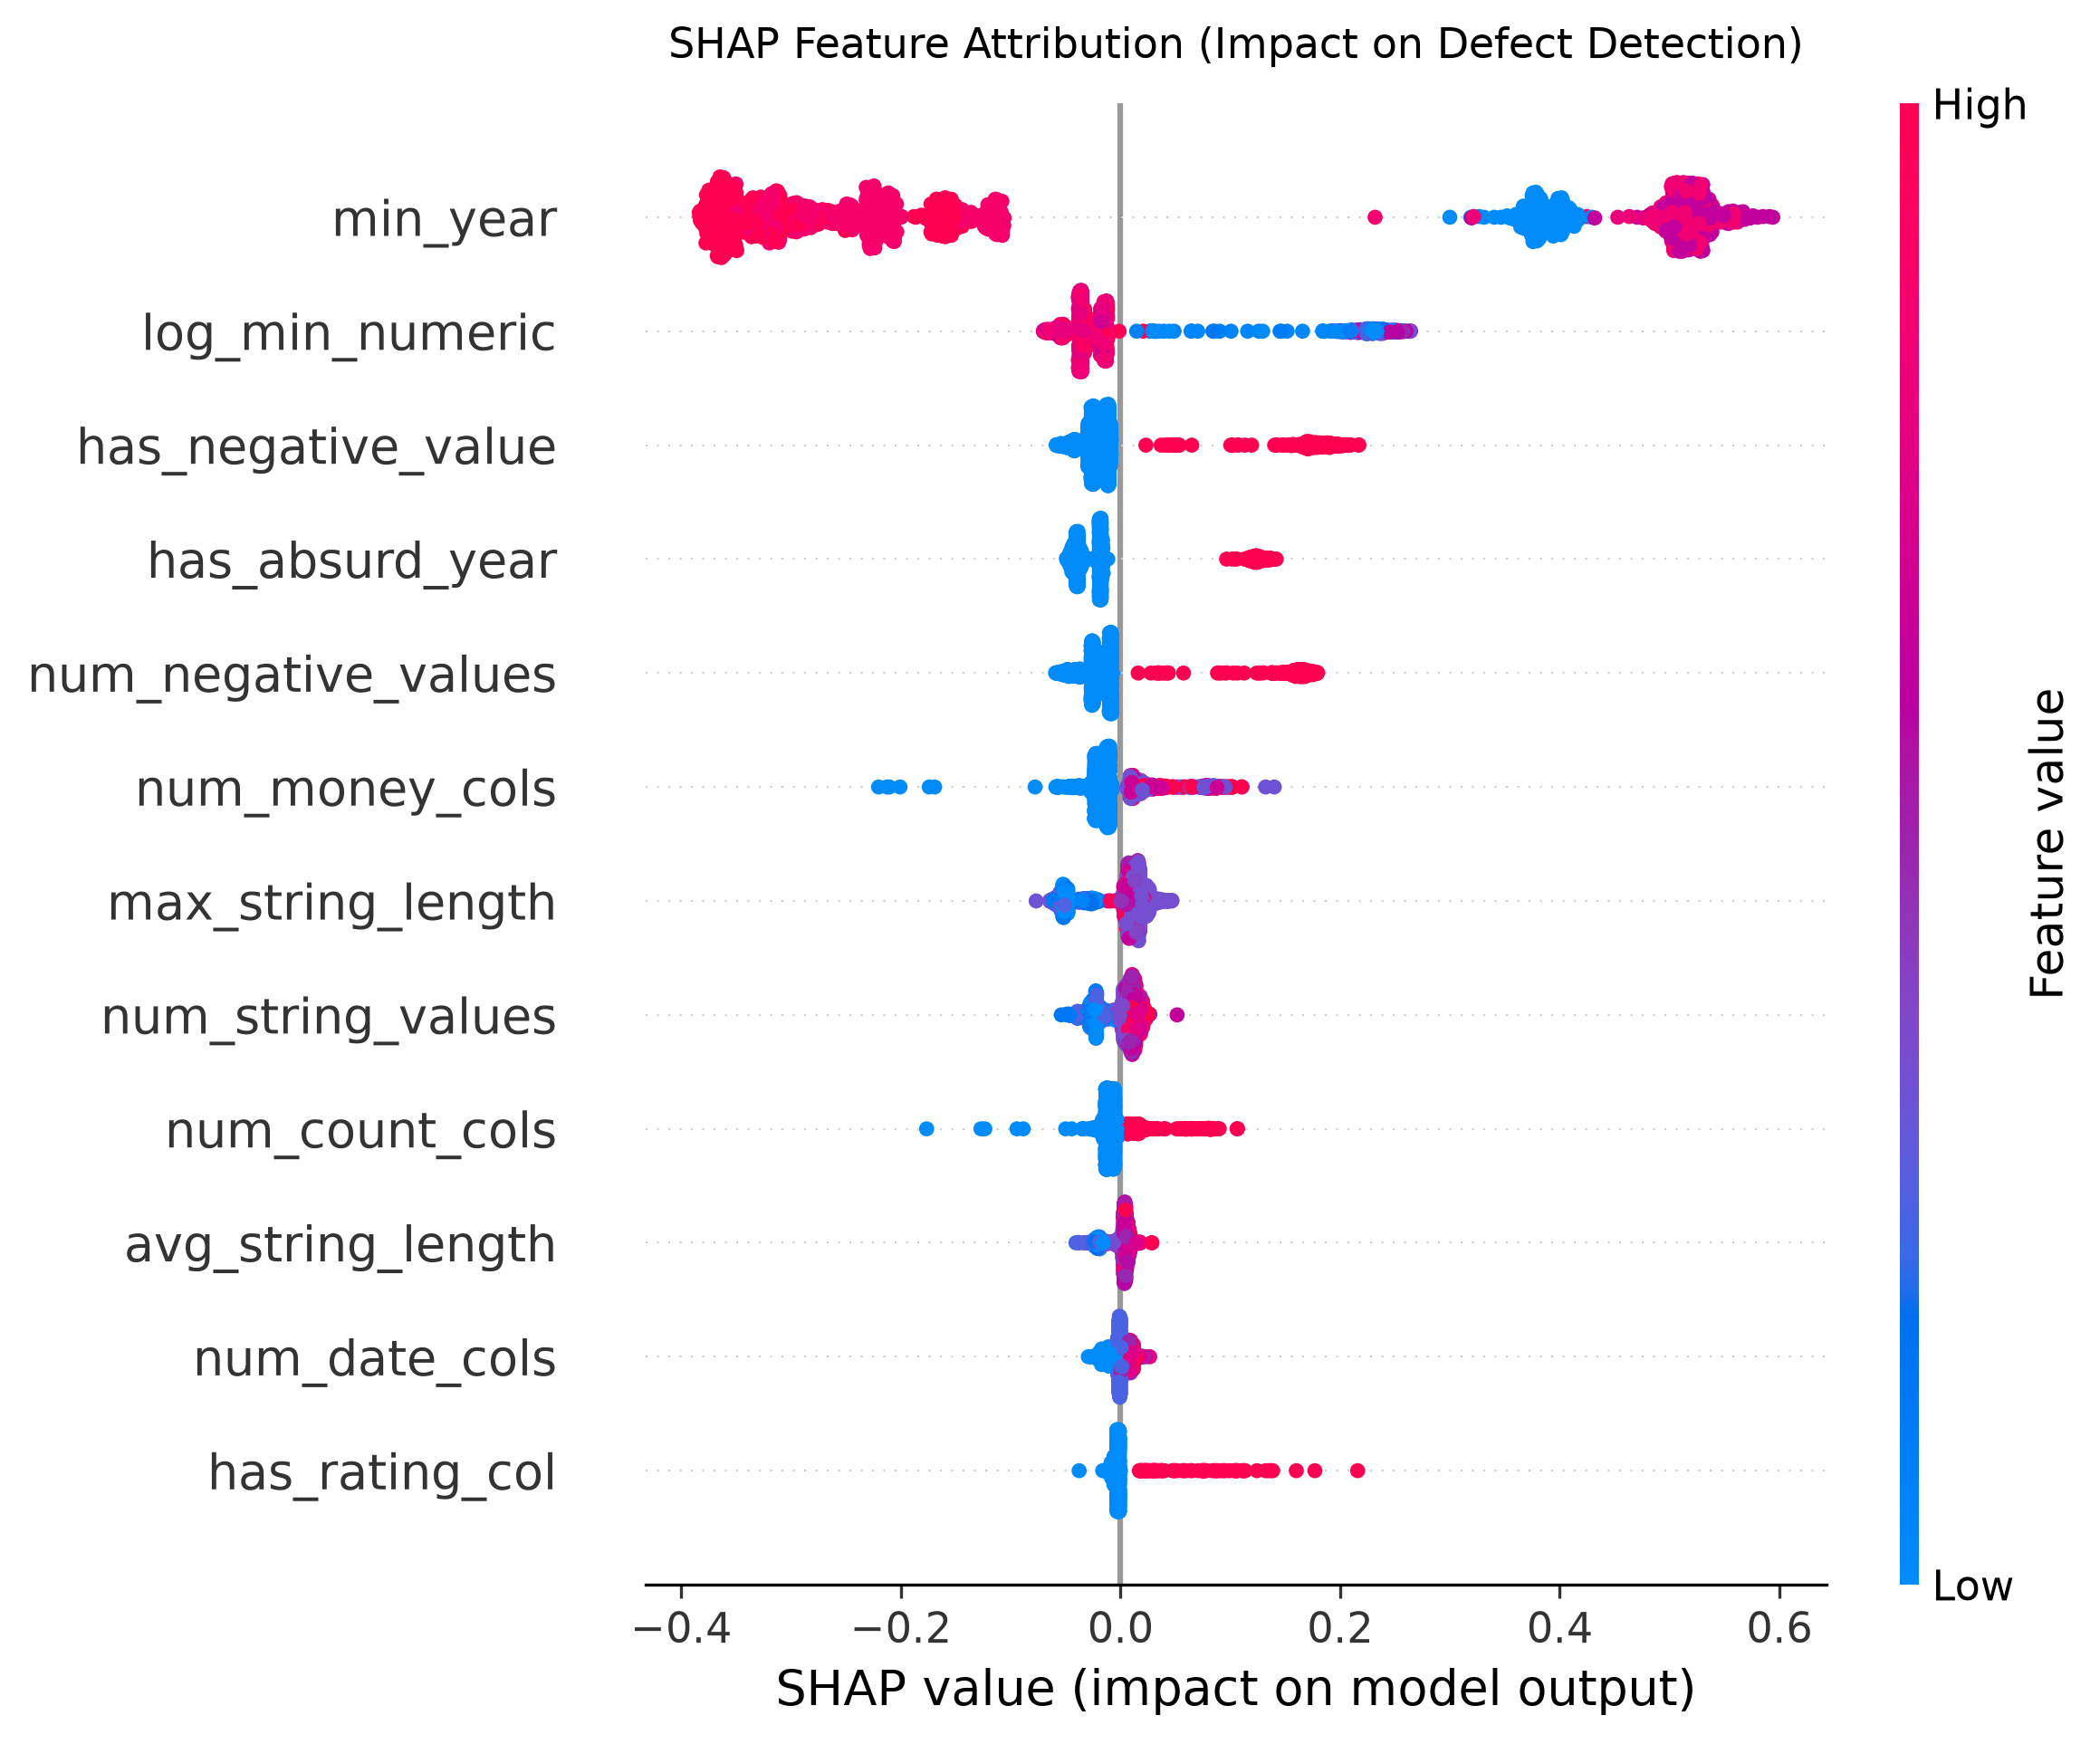
\includegraphics[width=\columnwidth]{figures/fig5_shap_beeswarm.png}
\caption{Global SHAP beeswarm distribution illustrating the directional impact of top-10 features on silent defect predictions.}
\label{fig:shap_beeswarm}
\end{figure}

\subsection{Case Studies: False Positives \& False Negatives}
\textbf{False Positives (395 / 31,015 clean test records, FPR = 1.27\%):} 
In \texttt{personal\_finance\_9}, the clean statement:
\begin{quote}
\small\texttt{INSERT INTO accounts VALUES (3, 1, 'Travel Credit Card', 'credit', -850.40, 'USD');}
\end{quote}
was assigned a corruption probability of 1.0. In business accounting logic, credit card balances and overdrafts are legitimately negative. The model over-relies on negative currency flags, mistaking legitimate financial debits for corruptions.

\textbf{False Negatives (1,030 / 119,369 corrupt records, FNR = 0.86\%):}
In \texttt{wishlist\_management\_1}, an out-of-bounds dish rating of \texttt{10.0} was assigned probability 0.013. We identified this as \textbf{Feature Masking}: the statement contained \texttt{restaurant\_id = 24}. Because aggregate row features record the global maximum numeric literal, the foreign key (24) masked the out-of-bounds rating (10.0).

\section{Remaining Limitations \& Project Plan}
\subsection{Current Difficulties \& Limitations}
\begin{itemize}
    \item \textbf{Feature Masking in Wide Tables:} Row-level aggregate extrema fail when high-magnitude primary/foreign keys overshadow subtle attribute corruptions.
    \item \textbf{Accounting Domain Semantics:} Legitimate negative numbers in finance and inventory decrement adjustments produce false alarms.
\end{itemize}

\subsection{Plan for Final Deliverables (Oct 19 -- Dec 7)}
\begin{enumerate}
    \item \textbf{Column-Aligned Feature Extraction:} Replace row-wide extrema with column-specific normalized Z-scores to resolve feature masking.
    \item \textbf{Contextual Disambiguation:} Incorporate categorical context (e.g., account type or adjustment reason) to eliminate false positives.
    \item \textbf{Interactive Demonstration Enhancement:} Maintain the Streamlit app (\texttt{demo\_app.py}) and record reproducible video demo.
\end{enumerate}

\bibliographystyle{IEEEtran}
\begin{thebibliography}{00}
\bibitem{wang2026awm} Z. Wang, C. Xu, B. Liu, Y. Wang, S. Han, Z. Yao, H. Yao, and Y. He, ``Agent World Model: Infinity Synthetic Environments for Agentic Reinforcement Learning,'' in \textit{Proc. Int. Conf. Mach. Learn. (ICML)}, 2026.
\bibitem{snowflake2026awm} Snowflake AI Research, ``AgentWorldModel-1K,'' Hugging Face Dataset, 2026. \url{https://huggingface.co/datasets/Snowflake/AgentWorldModel-1K}.
\bibitem{liu2008isolation} F. T. Liu, K. M. Ting, and Z.-H. Zhou, ``Isolation Forest,'' in \textit{Proc. IEEE Int. Conf. Data Min. (ICDM)}, 2008, pp. 413--422.
\bibitem{breiman2001random} L. Breiman, ``Random Forests,'' \textit{Mach. Learn.}, vol. 45, no. 1, pp. 5--32, 2001.
\bibitem{chen2016xgboost} T. Chen and C. Guestrin, ``XGBoost: A Scalable Tree Boosting System,'' in \textit{Proc. ACM SIGKDD Int. Conf. Knowl. Discov. Data Min.}, 2016, pp. 785--794.
\bibitem{lundberg2017shap} S. M. Lundberg and S.-I. Lee, ``A Unified Approach to Interpreting Model Predictions,'' in \textit{Adv. Neural Inf. Process. Syst. (NeurIPS)}, vol. 30, 2017.
\end{thebibliography}

\end{document}

